\documentclass[12pt]{article}

%\usepackage{algo}
\usepackage{tikz,fullpage,url,amssymb,amsmath,epsfig,color,xspace,alltt,mathtools}
\usetikzlibrary{shapes,chains,positioning}
\usepackage[pdftitle={CS 240 Assignment 2},%
pdfsubject={University of Waterloo, CS 240, Fall 2021},%
pdfauthor={MP}]{hyperref}
%\RequirePackage{pstricks,pst-node,pst-tree} % draw trees, requires using xetex
\newlength{\nodeLength}
\newcommand{\Node}{A}
\newcommand{\setnode}[1]{
	\settowidth{\nodeLength}{#1}
	\renewcommand{\Node}[1]{
		\Tcircle[name=#1]{\makebox[\nodeLength]{##1}}
	}
}
\setnode{99}

\newcommand{\ceil}[1]{\left\lceil #1 \right\rceil}
\newcommand{\floor}[1]{\left\lfloor #1 \right\rfloor}
\renewcommand{\thesubsection}{Problem \arabic{subsection}}

\begin{document}
	
	\begin{center}
		{\Large\bf Assignment 2 Problem 2}\\
		\vspace{3mm}
	\end{center}
	
	\definecolor{care}{rgb}{0,0,0}
	\def\question#1{\item[\bf #1.]}
	\def\part#1{\item[\bf #1)]}
	\newcommand{\pc}[1]{\mbox{\textbf{#1}}} % pseudocode
	
	
	
	%%%%%%%%%%%%%%%%%%%%%%%%%%%%%%%%%%%%%%%%%%%%%%%%%%%%%%%%%%%%%
	
		A \emph{pyramid} is a data structure similar to a heap that can be used
	to implement the priority queue ADT.
	
	As with a heap, a pyramid is defined by two properties:
	\begin{itemize}
		\item \textbf{Structural property}: A pyramid $P$ consists of $\ell \geq 0$ levels. The $i$th level, for $0\leq i < \ell$, 
		contains at most $i+1$ entries, indicated as
		$P_{i,j}$ for $0\leq j\leq i$. All levels but the last are completely
		filled, and the last level is left-justified.
		
		For example, the following diagram shows the structure of a pyramid with 4 levels and 9 nodes, labelled as described above.
		
		\begin{center}
			%\usetikzlibrary{positioning}
			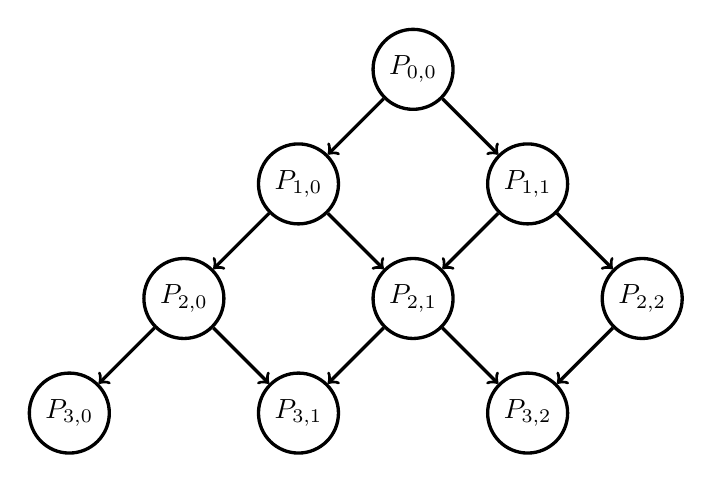
\begin{tikzpicture}[node distance=1cm,very thick]
				\node[circle,draw] (a0) {$P_{0,0}$};
				\node[circle,draw] (b0) [below left=of a0] {$P_{1,0}$};
				\node[circle,draw] (b1) [below right=of a0] {$P_{1,1}$};
				\node[circle,draw] (c0) [below left=of b0] {$P_{2,0}$};
				\node[circle,draw] (c1) [below right=of b0] {$P_{2,1}$};
				\node[circle,draw] (c2) [below right=of b1] {$P_{2,2}$};
				\node[circle,draw] (d0) [below left=of c0] {$P_{3,0}$};
				\node[circle,draw] (d1) [below right=of c0] {$P_{3,1}$};
				\node[circle,draw] (d2) [below right=of c1] {$P_{3,2}$};
				\path[->] (a0) edge (b0)
				(a0) edge (b1)
				(b0) edge (c0)
				(b0) edge (c1)
				(b1) edge (c1)
				(b1) edge (c2)
				(c0) edge (d0)
				(c0) edge (d1)
				(c1) edge (d1)
				(c1) edge (d2)
				(c2) edge (d2);
			\end{tikzpicture}
		\end{center}
		
		\item \textbf{Ordering property}: Any node $P_{i,j}$ has at most two
		\emph{children}: $P_{i+1,j}$ and $P_{i+1,j+1}$, if those nodes exist.
		The priority of a node is always greater than or equal to the priority
		of either child node.
		
		For example, the following diagram shows the ordering property for a pyramid with 4 levels and 9 nodes.  
		Priorities have been placed in the nodes and the arrows indicate ``$\geq$'' relationships.
		
		\begin{center}
			%\usetikzlibrary{positioning}
			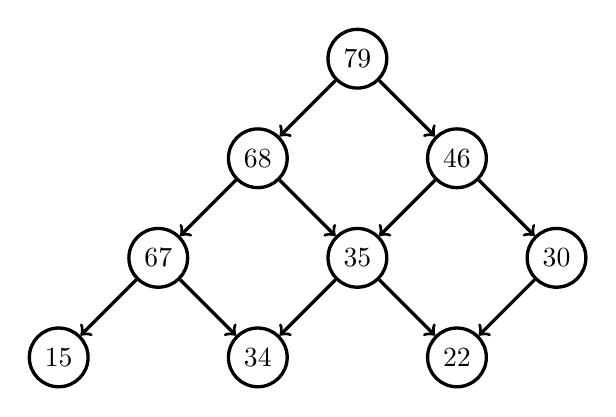
\begin{tikzpicture}[node distance=1cm,very thick]
				\node[circle,draw] (a0) {79};
				\node[circle,draw] (b0) [below left=of a0] {68};
				\node[circle,draw] (b1) [below right=of a0] {46};
				\node[circle,draw] (c0) [below left=of b0] {67};
				\node[circle,draw] (c1) [below right=of b0] {35};
				\node[circle,draw] (c2) [below right=of b1] {30};
				\node[circle,draw] (d0) [below left=of c0] {15};
				\node[circle,draw] (d1) [below right=of c0] {34};
				\node[circle,draw] (d2) [below right=of c1] {22};
				\path[->] (a0) edge (b0)
				(a0) edge (b1)
				(b0) edge (c0)
				(b0) edge (c1)
				(b1) edge (c1)
				(b1) edge (c2)
				(c0) edge (d0)
				(c0) edge (d1)
				(c1) edge (d1)
				(c1) edge (d2)
				(c2) edge (d2);
			\end{tikzpicture}
		\end{center}
	\end{itemize}
	
	\begin{itemize}
		\part{a}
		A pyramid $P$ with $n$ nodes can be stored in an array $A$ of size $n$,
		similar to an array-based heap. 
		For example, the top of the pyramid $P_{0,0}$ will be stored in $A[0]$, followed by level 1, then level 2, and so on.
		
		Give formulas for the array index that the following pyramid entries
		will have. Assume that $n$, $i$, and $j$ are such that all indicated
		pyramid nodes actually exist. You do not need to justify your answers.
		
		\begin{enumerate}
			\item $P_{i,j}$
			\item Left and right children of $P_{i,j}$
			\item Left and right parents of $P_{i,j}$
			\item (Bonus) Left and right children of the node corresponding to $A[i]$
		\end{enumerate}
		
		\part{b}
		Give upper and lower bounds for the number of nodes $n$ in a pyramid $P$
		with $\ell$ levels, where $\ell \geq 1$. For example, a pyramid with 2
		levels has at least 2 and at most 3 nodes. Your bounds should be tight.
		
		\part{c}
		Give pseudocode for the $\emph{delete-max}$ operation that takes a
		pyramid stored in an array $A$ of size $n$, removes the largest priority
		from the pyramid, and returns it.
		
		Explain why your algorithm preserves the structural and ordering properties
		of the pyramid; i.e. show that the resulting tree is a pyramid (according to
		the definition above).
		
		Show that your algorithm has time complexity $O(\sqrt{n})$.
		
		\part{d}
		Give pseudocode for the $\emph{insert}$ operation that takes a pyramid
		stored in an array $A$ of size $n$ and a priority $x$ and inserts the
		new element into the pyramid.
		
		Explain why your algorithm preserves the structural and ordering properties
		of the pyramid; i.e. show that the resulting tree is a pyramid (according to
		the definition above).
		
		Show that your algorithm has time complexity $O(\sqrt{n})$.
		
		\part{e}
		Consider the \emph{contains} problem: Given an array $A$ of size $n$
		and an number $x$, determine whether $x$ is an element of $A$.
		
		For example, if $A$ is sorted, the \emph{contains} problem can be solved in
		$O(\log n)$ time by using a binary search.
		
		Describe an efficient algorithm using pseudocode to solve the \emph{contains} problem when the input array $A$ is a pyramid as described above.  
		State and briefly describe the runtime of your algorithm.
		For full marks, your algorithm should run in $O(\sqrt{n})$.
		(Hint: A pyramid contains some sorted lists.)
		
	\end{itemize}
	\begin{center}
	\end{center}
	
	
	
	%%%%%%%%%%%%%%%%%%%%%%%%%%%%%%%%%%%%%%%%%%%%%%%%%%%%%%%%%%%%%
	Solution:
	\begin{itemize}
		\part{a}
		\begin{itemize}
			\part{1}
			For $P_{i,j}$, the index of it in the array should be $\frac{i(i+1)}{2}+j$
			\part{2}
			The index of the left child for $P_{i,j}$ should be $\frac{(i+1)(i+2)}{2}+j$\\
			The index of the right child for $P_{i,j}$ should be $\frac{(i+1)(i+2)}{2}+j+1$
			\part{3}
			The index of the left parent for $P_{i,j}$ should be $\frac{i(i-1)}{2}+j-1$\\
			The index of the rigtht parent for $P_{i,j}$  should be $\frac{i(i-1)}{2}+j$
			\part{4}
			Assume that $n=\floor{\frac{\sqrt{1+8i}-1}{2}}$ and $m=i-\frac{n(n+1)}{2}$\\
			Then,the left child for A[i] should be $\frac{(n+1)(n+2)}{2}+m$\\
			and the right child for A[i] should be $\frac{(n+1)(n+2)}{2}+m+1$
		\end{itemize}
		
		\part{b}
		Since for each level, the limit of nodes increases 1 comparing to the upper level,\\
		Thus, the upper bound of number of nodes for the pyramid $P$ with $l$ levels should be
		\begin{center}
			$1+2+...+l+(l+1)=\frac{(l+1)(l+2)}{2}$
		\end{center} 
		and the lower bound of number of nodes for the pyramid $P$ with $l$ levels should be
		\begin{center}
			$1+2+...+l+1=\frac{l(l+1)}{2}+1$
		\end{center}
		
		\part{c}
		The pseudocode for the delete-max:\\
		
		delete-max(A)\\
		A: The array that stores a pyramid\\
		i $\gets$ last(size)\\
		swap A[root()] and A[i]\\
		decrease size by 1\\
		fix-down(A,size,root())\\
		return A[i]\\
		
		where the pseducode for the fix-dwon(array,size,k) we called is as follow:\\
		
		fix-down(A,n,k)\\
		A: The array that stores a pyramid of size n\\
		k: The index corresponding to a node of the pyramid\\
		while k has children do\\
			\hphantom{1111} //Find the child with the larger key\\
			\hphantom{1111} j $\gets$ left child of k\\
			\hphantom{1111} if j is not last(n) and A[j+1] $>$ A[j]\\
			\hphantom{11111111} j $\gets$ j+1\\
			\hphantom{1111} if A[k] $\geq$ A[j]  break\\
			\hphantom{1111} swap A[j] and A[k]\\
			\hphantom{1111} k $\gets$ j\\
		
		For the constructural property of the new pyramid, we can focus on the constructural change during the delete-max(). What we do is just decreases the size of array by 1, which means that we just remove the rightmost element of the last level of the pyramid, which preserves the structural property since all the levels but the last are still completely filled, and the last level is left-justified.\\
		For the ordering property, similar to the operation on heap, we swap the last `leaf'(ie. the rightmost element in the last level) with the root before we decreases the size of pyramid. And after decreasing the size, we have a new structure which may not actually a pyramid since the root does not satifying the order property. For each swapping we focus on four nodes, let node a be the node that we want to do the fix-down, and its right child b, left child c, and node d be the common child of b and c.\\
		There are three possiblilities(actually there are 4, but two of them can be combined since the symmetry).
		\begin{itemize}
			\item case 1: if the key of a is greater than max\{b,c\}, then we are done. 
			\item case 2: if the key of a is less than min\{b,c\}, when we swap a with max\{b,c\}, the order property will not be affected when doing the next swap since a is also less than min\{b,c\}
			\item case 3: if the key of a is less than one of b and c but another is not. Suppose $a>b,a<c$, then we also have the inequality $d<b<a<c$. At this time we swap a and c. But we should also focus on the common child of b and c. Since if the next swap we swapping a and d, then since $a>b$, the structure will not satisfy the order property. But notice that since $a>d$, we will never swap a and d, therefore, the order property will still preserved since if the loop ends here, we are done, and if we swap it with another child of a, then it becomes another subproblem with the same situation.
		\end{itemize}
		For the compexity of the algorithm, consider the worst-case runtime.
		For a heap of height h, we have at least $1+2+3+...+h+1=\frac{(h+1)h}{2}+1$ nodes, and at most $1+2+...+(h+1)=\frac{(h+1)(h+2)}{2}$ nodes. Call n the number of nodes, we get $\frac{h^2}{2} \leq \frac{(h+1)h}{2}+1 \leq n \leq \frac{(h+1)(h+2)}{2} \leq (h+2)^2$ true for any binary tree. Taking square root then we get $\frac{h}{\sqrt{2}} \leq \sqrt{n} \leq h+2$. Rearranging, then we have $\sqrt{n}-2 \leq h \leq \sqrt{2}\sqrt{n}$. So, $h\in \Theta(\sqrt{n})$. The worst case is we loop through all levels once, therefore, the complexity of the algorithm should be $O(\sqrt{n})$\\
		Therefore, in conclusion, the order property and the structural property are both preserved. And the complexity of the algorithm should be $O(\sqrt{n})$.
		
		\part{d}
		The pseudocode for the insert:\\
		
		insert(x)\\
		increase size\\
		i $\gets$ last(size)\\
		A[i] $\gets$ x\\
		fix-up(A,i)\\
		
		where the pseducode for the fix-up(array,k) we called is as follow:\\
		
		fix-up(A,k)\\
		k: an index corresponding to a node of the pyramid\\
		while parent(k) exists and min\{A[left-parent(k)],A[right-parent(k)]\} $<$ A[k] do\\
		\hphantom{1111} i $\gets$ index of the smaller parent of k\\
		\hphantom{1111} swap A[k] and A[i]\\
		\hphantom{1111} k $\gets$ i\\
		
		For the structural property of the new pyramid, we can focus on the constructural change during the insert(). What we do is just increase the size of array by 1,w hcih means that we just add the rightmost element of the last level of the pyramid if the last level is not full, and if its full, we add a leftmost element on a new level. This preserves the structural property since all the levels but the last are still completely filled, and the last level is left-justified. The function returns ture if it finds the element, returns false otherwise.\\
		For the ordering property, similar to the operation on heap, we add the new element to the last node(ie. the leftmost element of the last level), and trying to fix upwards. Say the node that we currently want to fix up is a, then we find the smaller parent of a then swap it. The new structure satisfied with the ordering property since the greater parent is greater than the smaller parent , and the key of a is also greater than the key of the children of the smaller parent (since originally, the smaller parent is greater than its all children).
		In part c), we have already shown that the number of the level of the pyramid with size n is $\Theta(\sqrt{n})$. The worst worst-case for this algorithm also runs through each level once. Therefore, the complexity of the algorithm should be $O(\sqrt{n})$.\\	
			
		\part{e}
		The pseudocode for the contains:\\
		
		contains(x)\\
		A: The array that stores a pyramid
		i $\gets$ 0\\
		while i $\leq$ size do\\
		\hphantom{1111} j $\gets$ special-binary-search(i,size,x)\\
		\hphantom{1111} if j is true\\
		\hphantom{11111111} break\\
		\hphantom{1111} i $\gets$ right-child(i)\\
		
		Where the special-binary-search has some difference compared to the usual one. When the index + 1, we change it into index = left-child(index), and index - 1, we change it into index = right-parent(index), and the index of array's first element is input as a argument i given when call the function, and the index of last element is the index of last left-child from index i which is less than or equal to the size\\
		What this algorithm doing is we seperate the pyramid into some sorted list.(ie. let the pyramid has n filled level, then we seperate it into n different sorted list). And for any node, its right-parent, itself, and left-child(if exists) are in the same array, and they are consecutive. By doing the seperation, we have some sorted list with length 1(if the last level is not filled, then the shortest list should be 2),2,3,...,(h+1). And we apply the binary search on each of the list, then we can have the complexity of this algorithm:\\
		$\log 1 + \log 2 + ... + \log h = \log h!$, since $h\in \Theta(\sqrt {n})$\\
		then we have the complexity of this algorithm: $O(\log {(\sqrt{n}!)})$
	\end{itemize}
	
	
\end{document}